\chapter{Background}\label{chapter:basics}

Before getting into the details of our driver, some concepts central to any NVMe driver need to be explained in detail first: how communicating with PCIe devices works with Memory-Mapped I/O and Direct Memory Access, the NVMe specification itself, and our programming language of choice, Rust.

\section{PCIe}
TODO: chatgpt and inshallah

\section{Memory-Mapped I/O}
Memory-mapped I/O (MMIO) is a method of performing I/O operations between the CPU and peripheral devices with a computer. Configuring and accessing PCIe devices usually requires accessing its Base Address Registers (BARs) and memory; on PCIe devices, these are accessed through MMIO. The subsystem \texttt{uio} in Linux exposes the BARs, as well as other required interfaces as files in the pseudo-filesystem \texttt{sysfs}, which we map the BARs into main memory with \texttt{mmap(2)}. These are mapped as shared memory, so changes to the mapped memory are also written back to the file and vice-versa.

\section{Direct Memory Access}
Passing data between hosts and PCIe devices typically is done through the use of ``Direct Memory Access''(DMA); this allows peripheral devices to initiate accesses to main memory independently of the CPU. Enabling DMA needs to be done explicitly by setting the ``Bus Master'' bit to 1 in the PCI configuration space.

As PCIe devices access memory via physical addresses independently of the CPU, we require the buffers we use for DMA to stay in main memory. We can use \texttt{mlock(2)} to guarantee a memory page is locked in main memory, however the mapping is not static for 4 KiB pages, the standard page size on Linux. Instead, we make use of 2 MiB huge pages for this, where the physical addresses are pinned due to Linux not implementing page migration on 2 MiB huge pages \cite{user_space_net}.

Figuring out the physical address our memory mapped page is located at is done by examining the process page tables in the process' pagemap.


\section{Non-Volatile Memory Express}
Non-Volatile Memory Express (NVMe) itself ``is an open collection of standards and information to fully expose [\ldots] non-volatile memory in all types of computer environments''\footnote{\url{https://nvmexpress.org/about/}}. Relevant to the thesis is the NVMe specification, an open logical device interface specification for accessing non-volatile storage media attached via the PCIe bus. NVMe was designed to capitilise on the low latency and parallelism of SSDs, providing improvements over older storage interfaces such as SATA or SAS in terms of speed and latency. This specification defines several key components:

\begin{itemize}
    \item \textbf{NVMe commands}: the basic units of work that the host system uses to communicate with the NVMe device. These commands may involve I/O operations or administrative tasks. These submission entries contain the command opcode, an identifier, and values pertaining to the command, e.g. data pointers for read/write operations. The structure of such a command can be seen in \autoref{fig:nvme-queue}
    \item \textbf{Submission Queues (SQ)}: The host system places commands here to be processed by the NVMe device. Each NVMe device can support multiple SQs, enabling parallel command processing.
    \item \textbf{Completion Queues (CQ)}: The NVMe device places completion entries noticing that commands have to processed. Each completion queue is associated with a submission queue, however the specification allows multiple submission queues to be associated with a single completion queue.
\end{itemize}

The specification supports 1 Administrative submission and completion queue pair and up to 65535 I/O submission and completion queues, in theory allowing for high scalability and the ability to handle high volumes of I/O requests. Both the submission and completion queue operate as ring buffers, supporting up to 65536 entries and 65535 outstanding requests. Due to the command identifier being 16 bits in size, the NVMe controller in total supports up to 65536 outstanding requests at a time.

\subsection{Submitting and completing requests}
Submission and Completion Queues operate similarly to a Consumer-Producer pattern, e.g. in the case of an SQ, the host produces requests and adds them to the queue for the NVMe device to consume. Here we keep track of a $\texttt{tail}$ pointer as the producer, pointing to the next free slot and a $\texttt{head}$ pointer, pointing to the next slot to be consumed.

Submitting requests to the NVMe device is done by constructing and then inserting a submission entry into the queue and updating the corresponding doorbell register to the new $\texttt{tail}$ value, notifying the NVMe device of the newly submitted request. Upon completion, the NVMe controller will post a completion entry into the Completion Queue belonging to the Submission Queue. The completion entries contain the command identifier, the status of the operation, and other command specific information. After processing the completion, the host then updates the doorbell register of the completion queue to signal that the completion entry has been acknowledged and processed. Depending on how the driver configures the NVMe controller, the device may send an interrupt signal upon completion. Each SQ and CQ has its own doorbell register.

\begin{figure}
  \centering
    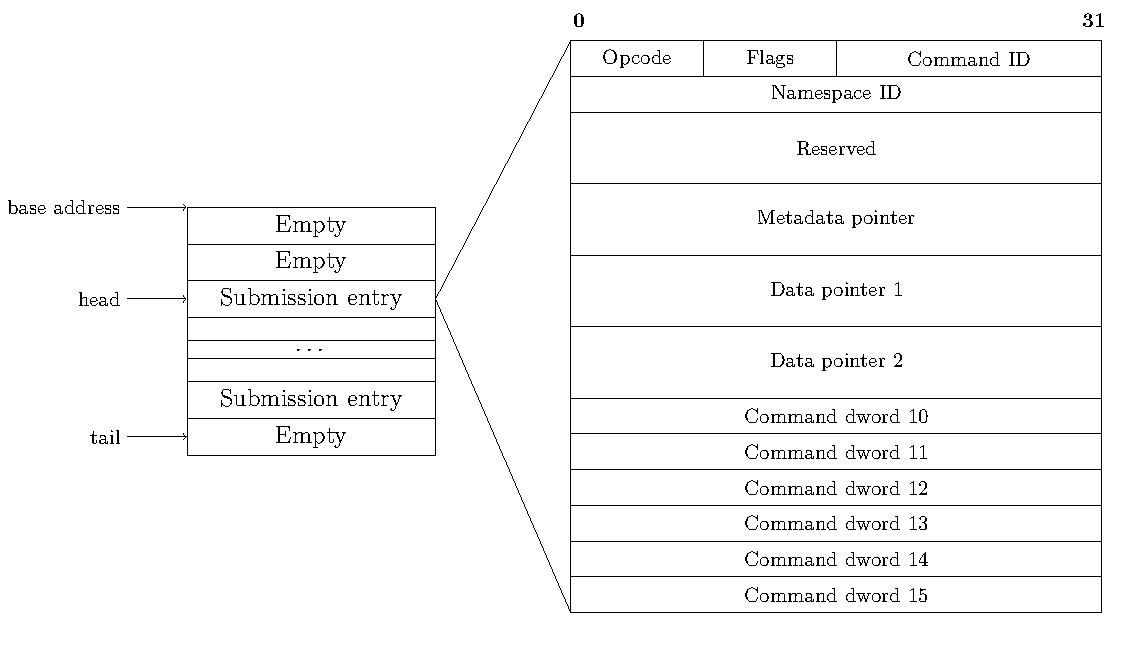
\includegraphics[width=\textwidth]{figures/nvme-queue}
    \caption{Example queue and structure of the NVMe submission entry}
    \label{fig:nvme-queue}
\end{figure}


For reading and writing depending on I/O size different data pointers are passed to the command. The addresses passed to the data pointers are called Physical Region Page (PRP), which is nothing more than a pointer to a physical memory page. There exists another data structure for describing data buffers called Scatter Gather Lists (SGL), however these are not supported by all NVMe SSD's while PRPs are.

For I/O operations less or equal to one page size (by default 4 KiB) we pass the physical address to Data pointer 1 (\texttt{d\_ptr[0]}). For requests up to two pages in size, we set \texttt{d\_ptr[0]} to the physical address and Data pointer 2 (\texttt{d\_ptr[1]}) to the address of the second block of data, e.g. \texttt{d\_ptr[0] + nvme\_page\_size} for contiguous memory. Once the I/O operation spans more than two pages, a pointer to a PRP list is passed to \texttt{d\_ptr[1]}. A PRP list is a list of PRP entries, where the last entry points to the next PRP list; essentially an array of pointers.

\begin{figure}
  \centering
    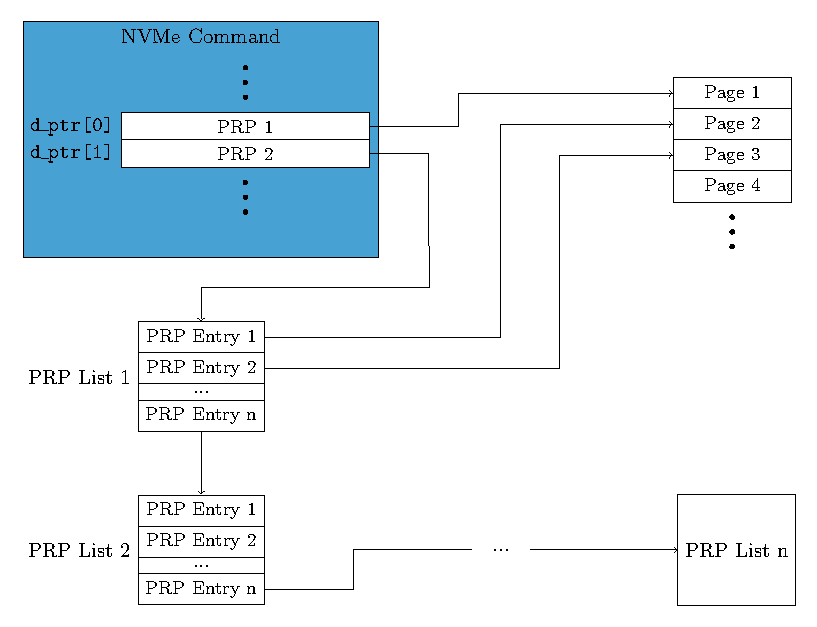
\includegraphics[width=\textwidth]{figures/prp-list}
    \caption{Visualisation of the PRP lists in NVMe commands}
    \label{fig:prp-list}
\end{figure}

% \begin{lstlisting}[float,language=Rust,label=lst:nvme_command,caption=NVMe command defined as a struct in Rust]
% #[repr(packed)]
% pub struct NvmeCommand {
%     pub opcode: u8,        // Command opcode
%     pub flags: u8,
%     pub c_id: u16,         // Command ID
%     pub ns_id: u32,        // Namespace ID
%     pub _rsvd: u64,        // Reserved
%     pub md_ptr: u64,       // Metadata pointer
%     pub d_ptr: [u64; 2],   // Data pointers
%     pub cdw10: u32,        // Command dwords; usage is command specific
%     pub cdw11: u32,
%     pub cdw12: u32,
%     pub cdw13: u32,
%     pub cdw14: u32,
%     pub cdw15: u32,
% } // 64 bytes
% \end{lstlisting}

% \begin{lstlisting}[float,language=Rust,label=lst:nvme_completion,caption=NVMe completion entry defined as a struct in Rust]
% #[repr(packed)]
% pub struct NvmeCompletion {
%     pub command_specific: u32,
%     pub _rsvd: u32, // Reserved
%     pub sq_head: u16, // Submission Queue head
%     pub sq_id: u16, // Submission Queue ID
%     pub c_id: u16, // Command ID
%     pub status: u16, // Status field
% } // 16 bytes
% \end{lstlisting}

\section{Rust}
While \texttt{C} remains the language used for the Linux kernel, it isn't necessarily the ideal language for driver development. In 2017, Cutler et al. analysed bugs in the Linux kernel which enabled arbitrary code execution and found out of 65, 40 bugs stemmed from invalid memory accesses, such as use-after-frees \cite{cutler}; it was found that 39 of these bugs stemmed from device drivers \cite{driver_lang}. Memory bugs remain amongst the most exploited vulnerabilities\footnote{\url{https://cwe.mitre.org/top25/archive/2023/2023_kev_list.html}}, and companies such as Google have begun to transition towards the use of memory-safe languages from \texttt{C} and \texttt{C++}.

Rust is a modern systems programming language with a focus on safety, speed and concurrency. It was designed to provide memory and thread safety guarantees through a unique onwership model without any performance pitfalls. These safety checks are done at compile time, eliminating common bugs like null-pointer dereferences and data races. Furthermore, Rust is a compiled language without a garbage collector, leading to much better performance compared to interpreted languages and less overhead compared to languages that have a garbage collector.

With all these factors in mind, Rust seems to be an ideal programming language for developing (user space) device drivers where safety and effiency are paramount.
